\section*{Autores}

\begin{wrapfigure}{l}{0.3\linewidth}

\includegraphics[width=\linewidth]{figuras/autor_felipe.jpg}
\end{wrapfigure}

\textbf{Felipe de Cássio Rocha Santos} é graduando em Engenharia de Computação pelo Inatel - 7Instituto Nacional de Telecomunicações. Estagiário no ICC - Inatel Competence Center, onde atua como desenvolvedor de \textit{software} e \textit{DevOps}. Entusiasta da tecnologia, é apaixonado por código aberto, \textit{containers}, GitHub e Linux.\newline

\begin{wrapfigure}{l}{0.3\linewidth}
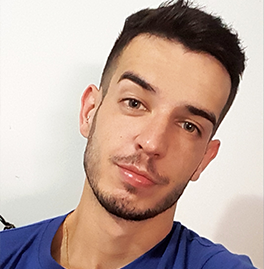
\includegraphics[width=\linewidth]{figuras/autor_igor.png}
\end{wrapfigure}

\textbf{Igor Galvão de Melo} é graduando em Engenharia de Computação pelo Instituto Nacional de Telecomunicações - Inatel. Estagiário na área de Engenharia de Vendas na empresa Ciena, e possui interesses na área de desenvolvimento de \textit{software}, vendas, planejamento e desenvolvimento de projetos.\newline

\begin{wrapfigure}{l}{0.3\linewidth}
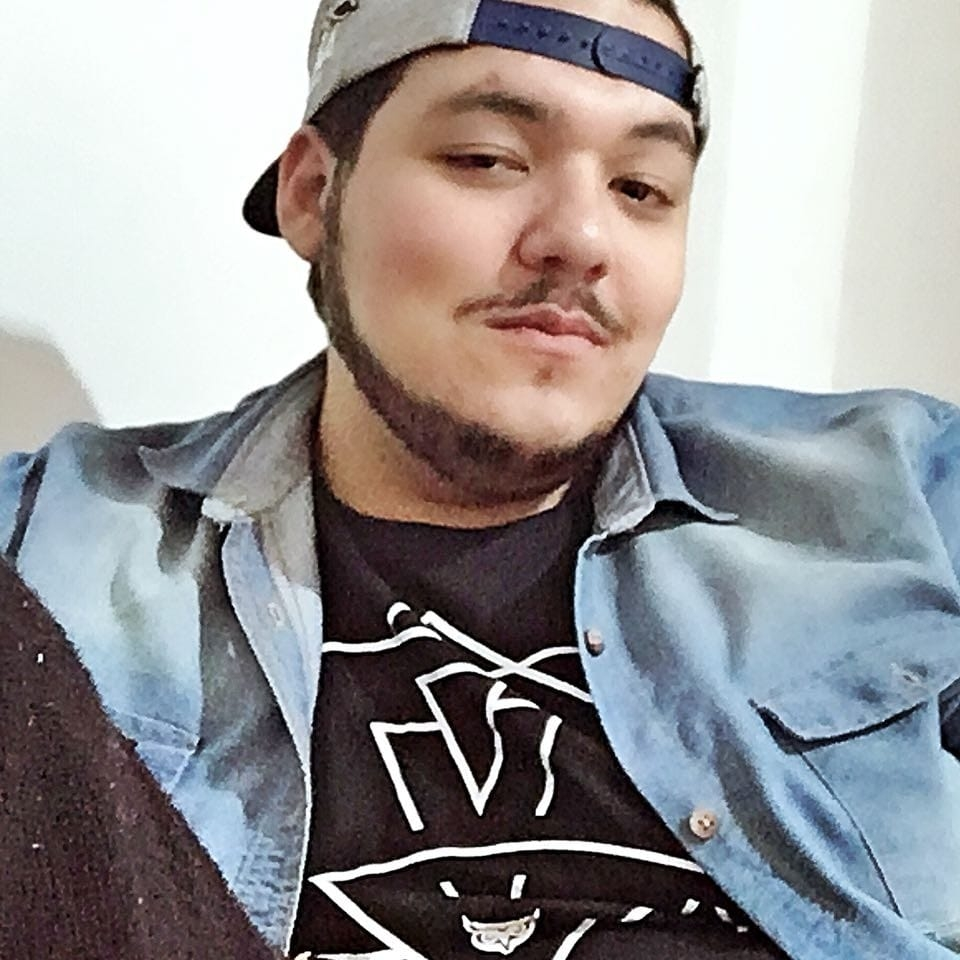
\includegraphics[width=\linewidth]{figuras/autor_lucas.jpg}
\end{wrapfigure}

\textbf{Lucas José Silva Corrêa} é graduando em Engenharia de Computação pelo Inatel - Instituto Nacional de Telecomunicações. Estagiário no Inatel Competence Center - ICC. Possui interesse nas áreas de tecnologia, DevOps e desenvolvimento de \textit{software}.\newline

\begin{wrapfigure}{l}{0.3\linewidth}
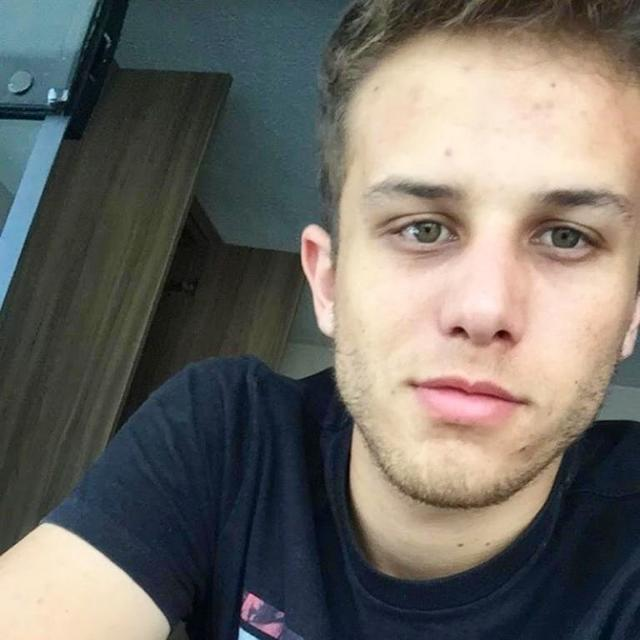
\includegraphics[width=\linewidth]{figuras/autor_thalis.jpg}
\end{wrapfigure}

\textbf{Thalis Andrade Oliveira de Souza} é graduando em Engenharia de Computação pelo Inatel - Instituto Nacional de Telecomunicações. Estagiário no ICC -  Inatel Competence Center, onde atua com desenvolvimento e testes de softwares e APIs. Possui interesse nas áreas de tecnologia, testes, SCRUM e desenvolvimento de \textit{software}.\newline

\begin{wrapfigure}{l}{0.3\linewidth}
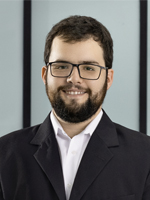
\includegraphics[width=\linewidth]{figuras/autor_marcelo.jpg}  
\end{wrapfigure}

\textbf{Marcelo Vinícius Cysneiros Aragão} é graduado em Engenharia de Computação pelo Instituto Nacional de Telecomunicações (Inatel) em 2014 e Mestre em Ciência e Tecnologia da Computação pela Universidade Federal de Itajubá em 2018. Trabalhou de 2011 a 2018 no Inatel Competence Center, mais recentemente como Especialista em Sistemas, onde atuou principalmente como desenvolvedor de soluções de Business Support Systems (BSS) em ambiente de integração contínua. É professor de disciplinas da graduação, como Inteligência Computacional e Redes Neurais, e coordenador do curso de pós-graduação em Desenvolvimento de Aplicações para Dispositivos Móveis e Cloud Computing. Possui interesse nas áreas de análise de algoritmos, desenvolvimento de \textit{software}, inteligência artificial, aprendizado de máquina e ciência de dados.
